
\documentclass[12pt]{article}


\usepackage{epsfig}
\usepackage{amsmath,amsthm}
\usepackage{listings}
\usepackage{graphicx}
\graphicspath{ {./images/} }


\newtheorem{lemma}{Lemma}
\newtheorem{theorem}{Theorem}


\usepackage{titlesec}
\titleformat{\section}
{\normalfont\Large\bfseries}{Question~\thesection:}{1em}{}

\newlength{\toppush}
\setlength{\toppush}{2\headheight}
\addtolength{\toppush}{\headsep}


\def\subjnum{Comp 150}
\def\subjname{Network Science}


\def\doheading#1#2#3{\vfill\eject\vspace*{-\toppush}%
  \vbox{\hbox to\textwidth{{\bf} \subjnum: \subjname \hfil Erli Cai}%
    \hbox to\textwidth{{\bf} Tufts University, Fall 2020 \hfil#3\strut}%
    \hrule}}


\newcommand{\htitle}[1]{\vspace*{1.25ex plus 1ex minus 0ex}%
\begin{center}
{\large\bf #1}
\end{center}} 



\begin{document}
\doheading{2}{title}{Homework 02}

\section{}
\subsection*{a}
blue nodes and black nodes represent people in different groups\\
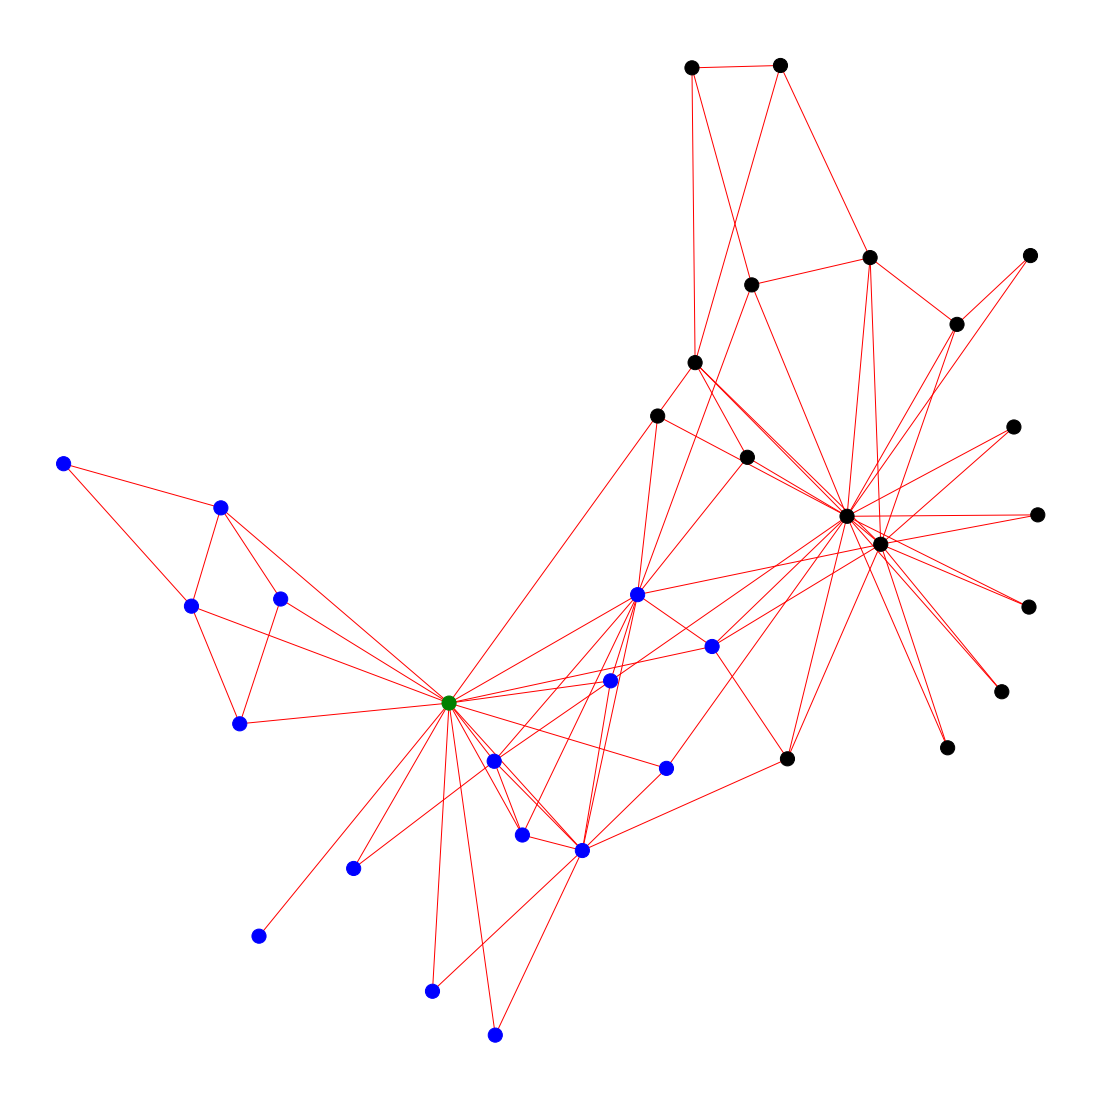
\includegraphics[width=\textwidth]{1.png}

\subsection*{b} The network is connected
\subsection*{c} Maximum degree is 17
\subsection*{d} The diameter of the network is 5
\subsection*{e} The clustering coefficient of the network 0.570(approximated to 3 decimal degrees)
\subsection*{f}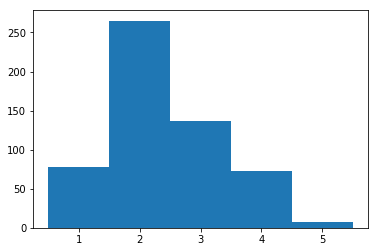
\includegraphics[scale = 0.7]{2.png}
\subsection*{g}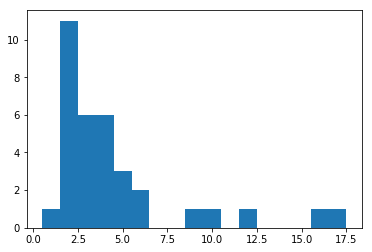
\includegraphics[scale = 0.7]{3.png}
\subsection*{h} The most central node is colored green in the graph in question(b)\\
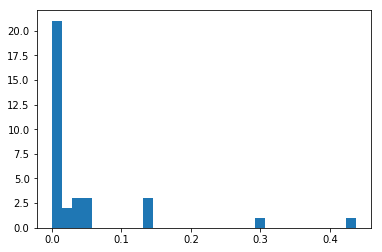
\includegraphics[scale = 0.7]{4.png}
\subsection*{i}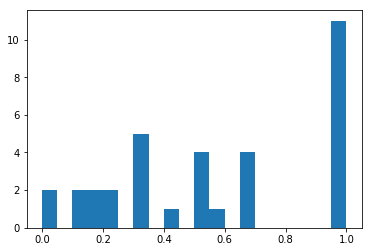
\includegraphics[scale = 0.7]{5.png}
\pagebreak


\section{}
\subsection*{a}
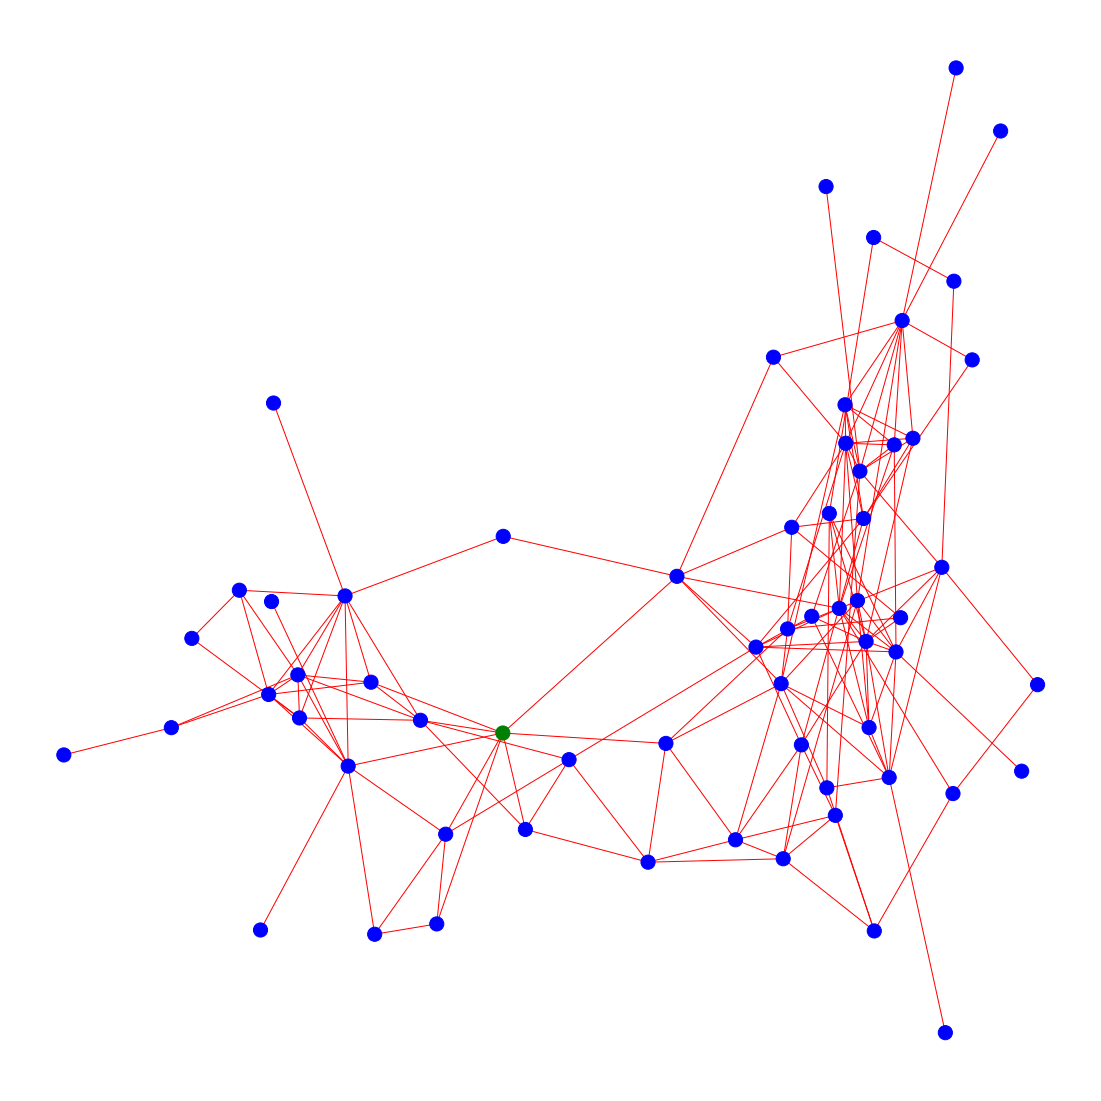
\includegraphics[width=\textwidth]{11.png}
\pagebreak
\subsection*{b} The network is connected
\subsection*{c} Maximum degree is 12
\subsection*{d} The diameter of the network is 8
\subsection*{e} The clustering coefficient of the network 0.259(approximated to 3 decimal degrees)
\subsection*{f}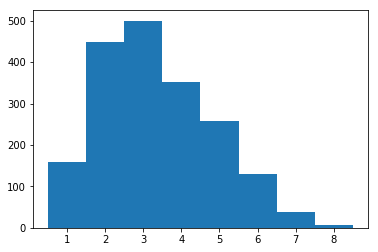
\includegraphics[scale = 0.7]{12.png}
\subsection*{g}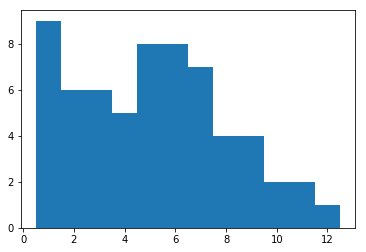
\includegraphics[scale = 0.7]{13.png}
\subsection*{h} The most central node is colored green in the graph in question(b)\\
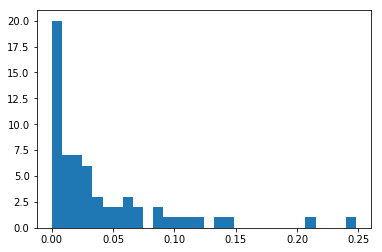
\includegraphics[scale = 0.7]{14.png}
\subsection*{i}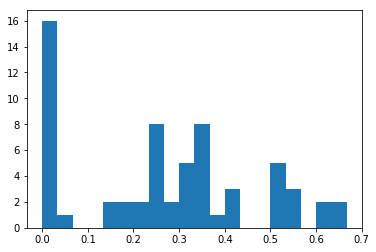
\includegraphics[scale = 0.7]{15.png}
\pagebreak


\section{}
\subsection*{a}
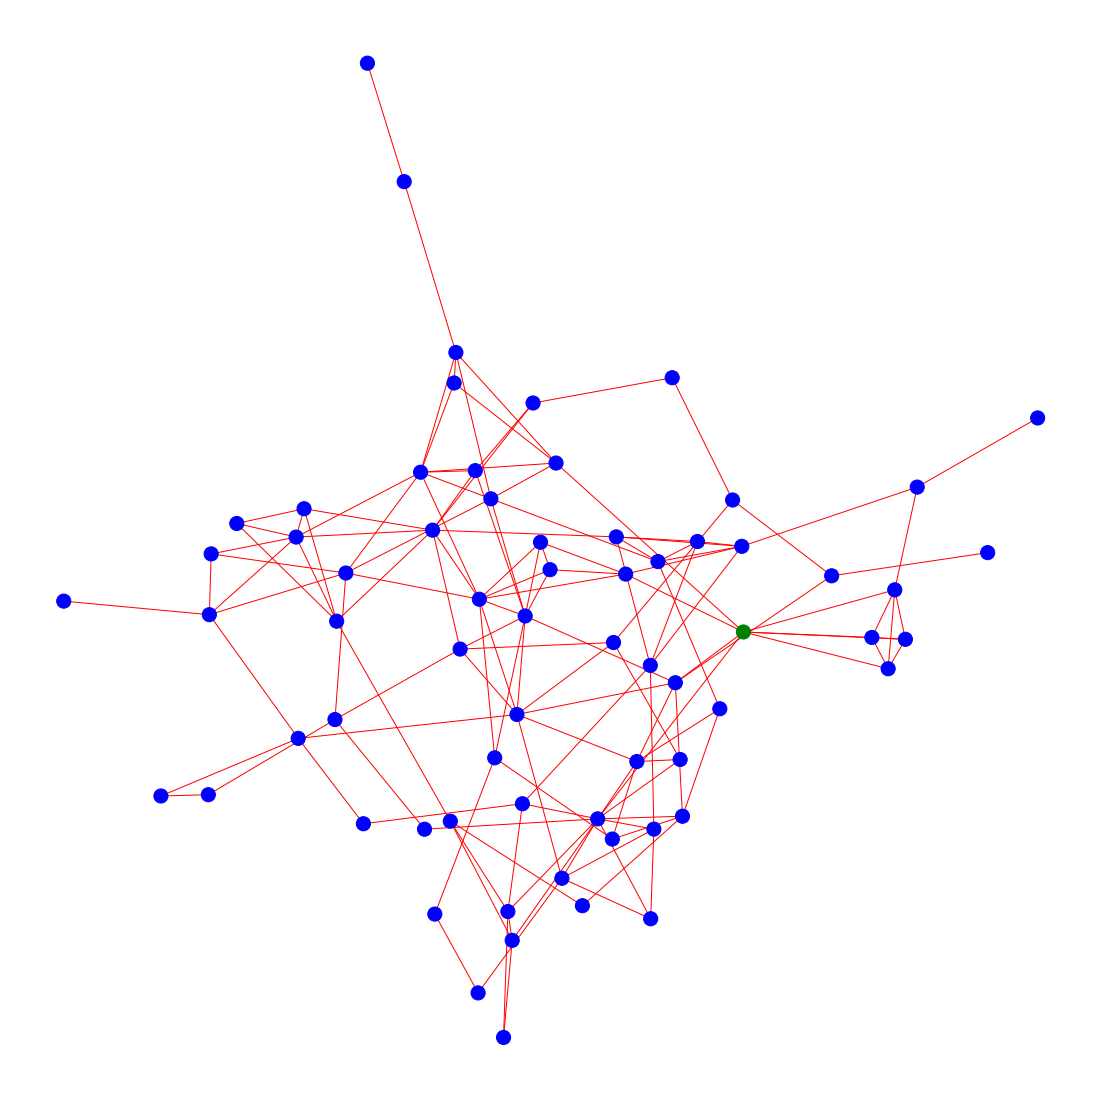
\includegraphics[width=\textwidth]{21.png}
\pagebreak
\subsection*{b} The network is connected
\subsection*{c} Maximum degree is 11
\subsection*{d} The diameter of the network is 7
\subsection*{e} The clustering coefficient of the network 0.310(approximated to 3 decimal degrees)
\subsection*{f}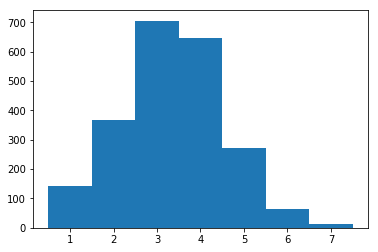
\includegraphics[scale = 0.7]{22.png}
\subsection*{g}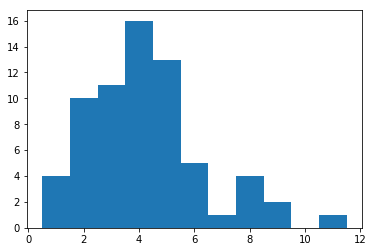
\includegraphics[scale = 0.7]{23.png}
\subsection*{h} The most central node is colored green in the graph in question(b)\\
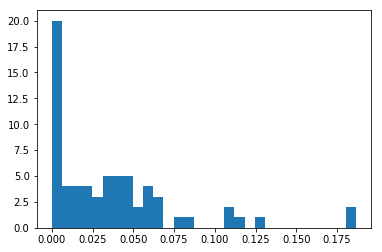
\includegraphics[scale = 0.7]{24.png}
\subsection*{i}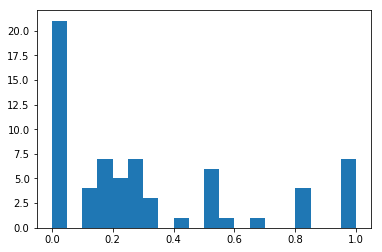
\includegraphics[scale = 0.7]{25.png}
\pagebreak





\end{document}


